\documentclass[a4paper,12pt]{article}

%%% Работа с русским языком
\usepackage{cmap}					% поиск в PDF
\usepackage{mathtext} 				% русские буквы в формулах
\usepackage[T2A]{fontenc}			% кодировка
\usepackage[utf8]{inputenc}			% кодировка исходного текста
\usepackage[english,russian]{babel}	% локализация и переносы
\usepackage{xcolor}
\usepackage{hyperref}
 % Цвета для гиперссылок
\definecolor{linkcolor}{HTML}{799B03} % цвет ссылок
\definecolor{urlcolor}{HTML}{799B03} % цвет гиперссылок

\hypersetup{pdfstartview=FitH,  linkcolor=linkcolor,urlcolor=urlcolor, colorlinks=true}

%%% Дополнительная работа с математикой
\usepackage{amsfonts,amssymb,amsthm,mathtools} % AMS
\usepackage{amsmath}
\usepackage{icomma} % "Умная" запятая: $0,2$ --- число, $0, 2$ --- перечисление

%% Номера формул
%\mathtoolsset{showonlyrefs=true} % Показывать номера только у тех формул, на которые есть \eqref{} в тексте.

%% Шрифты
\usepackage{euscript}	 % Шрифт Евклид
\usepackage{mathrsfs} % Красивый матшрифт

%% Свои команды
\DeclareMathOperator{\sgn}{\mathop{sgn}}

%% Перенос знаков в формулах (по Львовскому)
\newcommand*{\hm}[1]{#1\nobreak\discretionary{}
{\hbox{$\mathsurround=0pt #1$}}{}}
% графика
\usepackage{graphicx}
\graphicspath{{pictures/}}
\DeclareGraphicsExtensions{.pdf,.png,.jpg}
\author{Бурмашев Григорий, БПМИ-208}
\title{Математические структуры, кр -- 1}
\date{\today}
\begin{document}
\maketitle
\section*{Номер 1}
\begin{center}
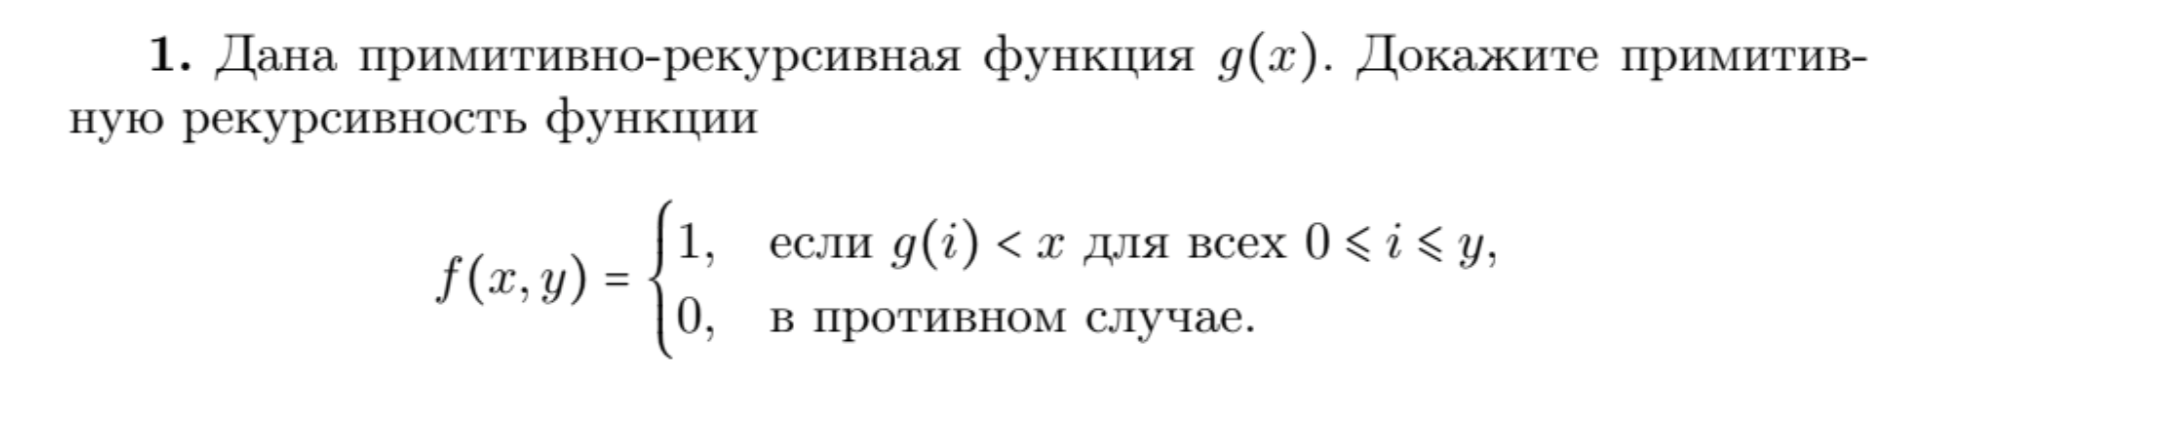
\includegraphics[scale=0.4]{1.png}
\end{center}
\def\dotminus{\mathbin{\ooalign{\hss\raise1ex\hbox{.}\hss\cr
  \mathsurround=0pt$-$}}}
На семинаре доказали, что $\text{sg}(x)$ --  примитивно-рекурсивная функция, возьмем это за основу для доказательства, поскольку $f(x, y)$ очень похожа на неё. Тогда введём вспомогательную функцию:
\[
h(x, i) = \begin{cases}
1, \; \text{ если } g(i) < x \\
0, \; \text{ в противном случае. } 
\end{cases}
\]
Тогда можем выразить ее через  $\text{sg}(x)$ и $x \dotminus y$:
\[
h(x, i) = \text{sg} (x \dotminus g(i))
\] 
В номере 3 из листка 3 доказали, что функции $\text{sg}(x)$ и  $x \dotminus y$ примитивно-рекурсивные, $g(x)$ -- примитивно-рекурсивная по условию задачи, а значит $h(x, i)$ -- тоже примитивно-рекурсивная функция как композиция. Но мы хотим $f(x, y)$, для этого замечаем, что мы можем выразить её через $h(x, i)$, просто добавив условие про $ 0 \leq i \leq y$:
\[
f(x, y) = \prod_{i \leq y} h(x, i)
\]
А теперь вспоминаем про номер 6 из листка 3,  где доказали замкнутость относительно мультиплицирования. 
Отсюда получаем, что $f(x, y)$ -- примитивно-рекурсивная функция.
\begin{center}
\textbf{Ч.Т.Д} 
\end{center}
\clearpage
\section*{Номер 2}
\begin{center}
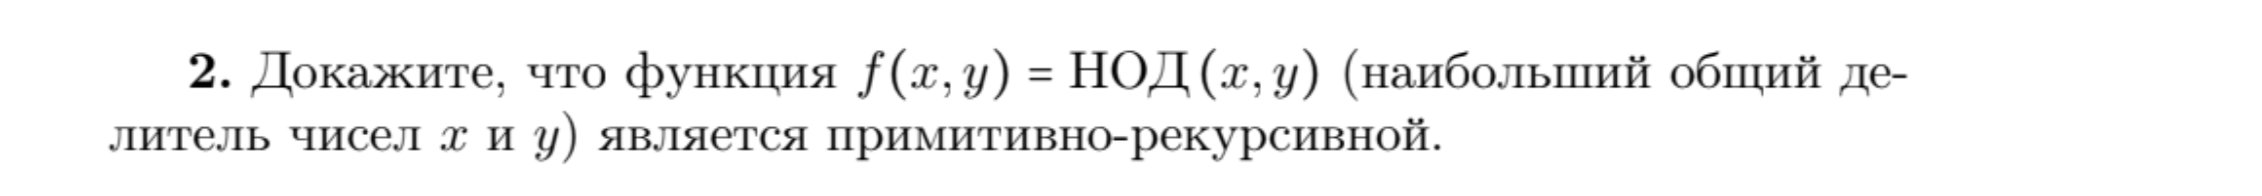
\includegraphics[scale=0.4]{2.png}
\end{center}
Обозначим для удобства:
\[
f(x, y) = \text{НОД}(x, y) = \gcd(x, y) 
\]
Замечаем:
\[
\gcd(x, 0) = x
\]
\[
\gcd(x, y) = \gcd \left(
\max(x, y) - \min(x, y), \min(x, y)
\right)
\]
Из семинара знаем, что функции $\min(x, y), \max(x, y), x - y$ примитивно-рекурсивны, а значит мы смогли представить нашу функцию $f(x, y)$ как суперпозицию примитивно-рекурсивных функций, значит $f(x, y)$ -- примитивно рекурсивна.
\begin{center}
\textbf{Ч.Т.Д} 
\end{center}
К тому же можно заметить (не очень формально), что функцию НОД мы можем определить как рекурсивный алгоритм с помощью ЯП. На семинаре доказывали, что $\text{rm}(x, y)$ -- остаток от деления $x$ на $y$ является примитивно-рекурсивной функцией. Пример кода рекурсивного вычисления НОД:
\begin{center}
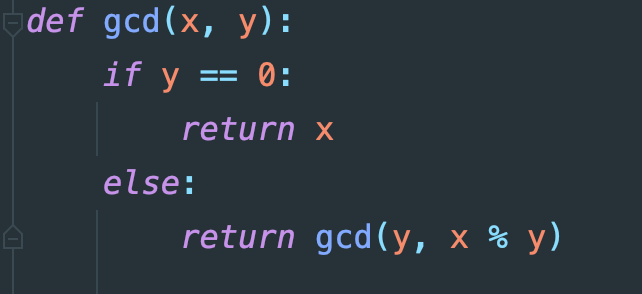
\includegraphics[scale=0.8]{5.png}
\end{center}
\clearpage
\section*{Номер 3}
\begin{center}
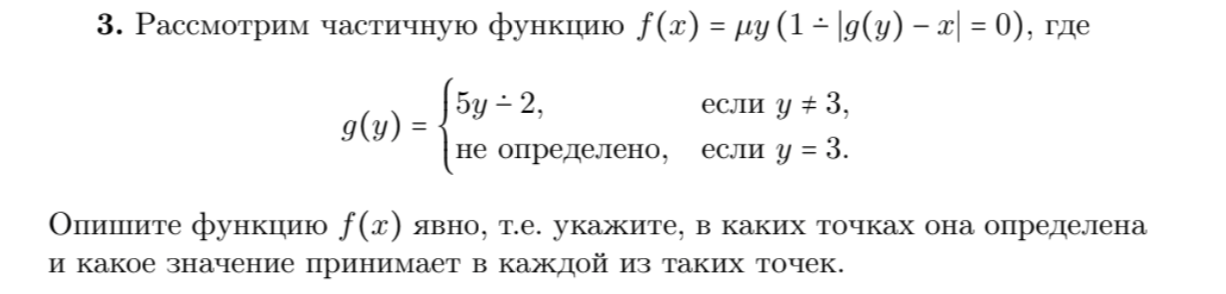
\includegraphics[scale=0.4]{3.png}
\end{center}
Разберемся с $\mu y()$:
\[
1 \dotminus |g(y) - x| = \begin{cases}
1 - |g(y) - x|, \; \text{ если } 1 \geq |g(y) - x|  \\
0, \; \text{ иначе } 
\end{cases}
\]
Тогда:
\[
1 \dotminus |g(y) - x| = 0  \sim |g(y) - x| \geq 1
\]
Тогда предположим, что $f(x) = 0 $ и посмотрим, что происходит в таком случае:
\[
f(x) = 0 \rightarrow y = 0 \rightarrow |g(0) - x| \geq 1 \rightarrow |0 - x| \geq 1 \rightarrow x \geq 1
\]
Получаем, что $f(x) = 0 \;  \forall \; x \; \geq 1$. Еще интересует $x = 0$, в этой точке:
\[
f(0) = \mu y (1 \dotminus |g(y) - 0| = 0)
\]
\[
f(0) = \mu y (1 \dotminus |g(y)| = 0)
\]
\[
f(0) = \mu y (1 \dotminus g(y) = 0)
\]
Отсюда:
\[
y = 1
\]
Значит:
\[
f(x) = \begin{cases}
1, \; x = 0 \; \\
0, \; \text{ иначе }
\end{cases}
\]
\begin{center}
\textbf{Ответ: } 
\[
f(x) = \begin{cases}
1, \; x = 0 \; \\
0, \; \text{ иначе }
\end{cases}
\]
\end{center}
\clearpage
\section*{Номер 4}
\begin{center}
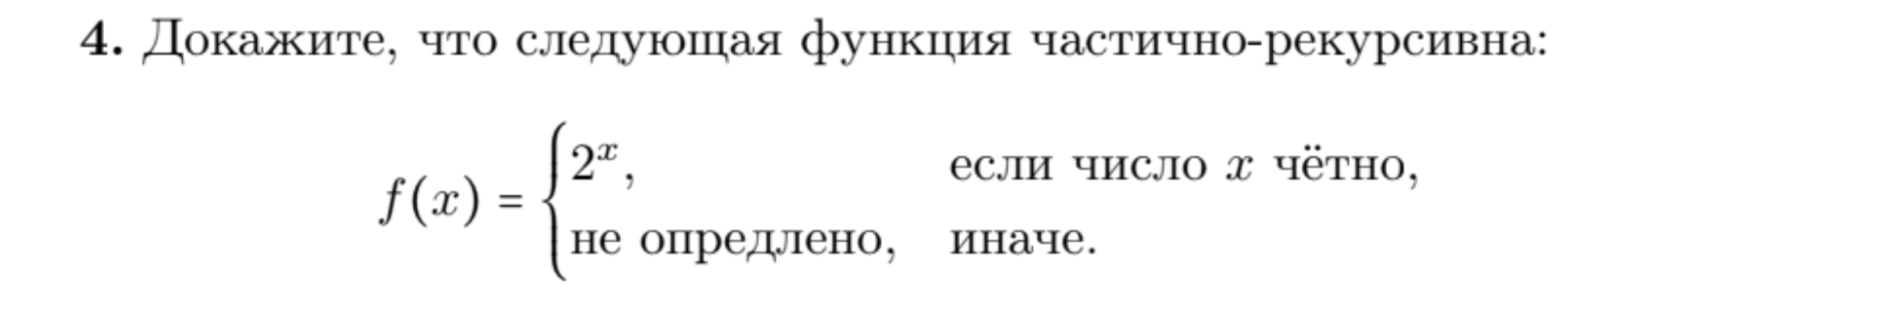
\includegraphics[scale=0.4]{4.png}
\end{center}
Воспользуемся задачей 8 (пункт 4) из листка 4. Для этого представим нашу функцию в другом виде, чтобы было удобнее, знаем, что:
\[
2^x = 4^{\frac{x}{2}}
\]
Тогда:
\[
f(x) = 
\begin{cases}
4^{\frac{x}{2}}, \text{ если число } x \text{ чётно} \\
\text{не определено, иначе.}
\end{cases}
\]
Делаем аналогично указанной выше задаче и кладем:
\[
\mu z \left(
h(x, 2, z) = 0
\right)
\]
Где:
\[
h(x, 2, z) = |x - 2 \cdot z| 
\]
Это в точности будет задавать:
\[
\frac{x}{2} = 
\begin{cases}
\frac{x}{2}, \text{ если } x \text{ делится на } 2 \text{ без остатка } \\
\text{не определено, иначе.} 
\end{cases}
\]
$x$ делится на $2$ без остатка по определению означает, что $x$ -- четно, а значит нашу функцию мы можем представить как:
\[
f(x) = 4^{\mu z \left(
h(x, 2, z) = 0
\right)}
\]
Ну и получаем, что наша функция это композиция примитивно-рекурсивной ($4^x$, т.е степень) и частично-рекурсивной (из задачи 8 пункт 4) функций, а значит $f(x)$ -- частично-рекурсивна
\begin{center}
\textbf{Ч.Т.Д} 
\end{center}
\end{document}
